%\listfiles
\documentclass[tg]{mdtuffs}
% um tipo específico de monografia pode ser informado como parâmetro opcional:
%\documentclass[tese]{mdtuffs}
% a opção `openright' pode ser usada para forçar inícios de capítulos
% em páginas ímpares
% \documentclass[openright]{mdtuffs}
% para gerar uma versão frente-e-verso, use a opção 'twoside':
% \documentclass[twoside]{mdtuffs}
%\usepackage{hyperref}	
%\usepackage{breakurl}
\usepackage[T1]{fontenc}        % pacote para conj. de caracteres correto
\usepackage{fix-cm} %para funcionar corretamente o tamanho das fontes da capa
\usepackage{times, color,xcolor}       % pacote para usar fonte Adobe Times e cores
\usepackage[utf8]{inputenc}   % pacote para acentuação
\usepackage{graphicx}  % pacote para importar figuras
\usepackage{caption}

%\usepackage[brazil]{babel}   
\usepackage{enumerate}
\usepackage{amsmath,latexsym,amssymb} %Pacotes matemáticos
\usepackage[%hidelinks%, 
            bookmarksopen=true,linktoc=none,colorlinks=true,
            linkcolor=black,citecolor=black,filecolor=magenta,urlcolor=blue,
            pdftitle={Extração de características para identificação de textos ofensivos},
            pdfauthor={Nome Autor Sobrenome},
            pdfsubject={Projeto/Trabalho de Conclusão de Curso},
            pdfkeywords={Monografia, Modelo, LaTeX}
            ]{hyperref} %hidelinks disponível no pacote hyperref a partir da versão 2011-02-05  6.82a
%Nesse caso, hidelinks retira os retângulos em volta dos links das referências

%Definição de minha autoria pra funcionar as XML
%\def\lnl#1#2{{\scriptsize\bfseries #1}\hspace{#2em}}
\usepackage{setspace}
%---------------------------------------------------
% Definições dos XML
%---------------------------------------------------
\usepackage{verbatim}
\usepackage{listings}
\usepackage{multicol}
%\usepackage[usenames,dvipsnames]{color}
	%\def\mlnl#1#2{{\scriptsize\bfseries #1}\hspace{#2em}}

%---------------------------------------------------
% Definições dos Algoritmos
%---------------------------------------------------
	\usepackage[portuguese,ruled,linesnumbered]{algorithm2e}
	\usepackage{etoolbox}
	\makeatletter
	\patchcmd{\@algocf@start}{%
		\begin{lrbox}{\algocf@algobox}%
	}{%
	  \rule{0.\textwidth}{\z@}%
	  \begin{lrbox}{\algocf@algobox}%
	  \begin{minipage}{1.\textwidth}%
	}{}{}
	\patchcmd{\@algocf@finish}{%
	  \end{lrbox}%
	}{%
	  \end{minipage}%
	  \end{lrbox}%
	}{}{}
	\makeatother

	\SetAlFnt{\tt}
	
	\SetKwFunction{FRecurs}{FnRecursive}%
%-------------------------------------------------

     
\sloppy
%%Margens conforme MDT 1ª edição, arrumar diretamente no mdtuffs.cls para funcionar a opção twoside *PENDENTE*
\usepackage[inner=30mm,outer=20mm,top=30mm,bottom=20mm]{geometry} 

%==============================================================================
% Se o pacote hyperref foi carregado a linha abaixo corrige um bug na hora
% de montar o sumário da lista de figuras e tabelas
% Se o pacote não foi carregado, comentar a linha %
%==============================================================================
%%=============================================================================
%% Trampa para corrigir o bug do hyperref que redefine o caption das figuras e das
%% tabelas, n�o colocando o nome ``Figura'' antes do n�mero do mesmo na lista
%%=============================================================================

\makeatletter

\long\def\@caption#1[#2]#3{%
  \expandafter\ifx\csname if@capstart\expandafter\endcsname
                  \csname iftrue\endcsname
    \global\let\@currentHref\hc@currentHref
  \else
    \hyper@makecurrent{\@captype}%
  \fi
  \@ifundefined{NR@gettitle}{%
    \def\@currentlabelname{#2}%
  }{%
    \NR@gettitle{#2}%
  }%
  \par\addcontentsline{\csname ext@#1\endcsname}{#1}{%
    \protect\numberline{\csname fnum@#1\endcsname ~-- }{\ignorespaces #2}%
  }%
  \begingroup
    \@parboxrestore
    \if@minipage
      \@setminipage
    \fi
    \normalsize
    \expandafter\ifx\csname if@capstart\expandafter\endcsname
                    \csname iftrue\endcsname
      \global\@capstartfalse
      \@makecaption{\csname fnum@#1\endcsname}{\ignorespaces#3}%
    \else
      \@makecaption{\csname fnum@#1\endcsname}{%
        \ignorespaces
        \ifHy@nesting
          \expandafter\hyper@@anchor\expandafter{\@currentHref}{#3}%
        \else
          \Hy@raisedlink{%
            \expandafter\hyper@@anchor\expandafter{%
              \@currentHref
            }{\relax}%
          }%
          #3%
        \fi
      }%
    \fi
    \par
  \endgroup
}

\makeatother

%==============================================================================
% Identificação do trabalho
%==============================================================================
\title{Extração de características para identificação de discurso de ódio em documentos}

\author{de Lima Pinto}{Cleiton}
%Descomentar se for uma "autora"
%\autoratrue

\course{Curso de Ciência da Computação}
\altcourse{Curso de Ciência da Computação}

%não usado por enquanto
\institute{Ciência da Computação}
\degree{Bacharel em Ciência da Computação}

% Número do TG (verificar na secretaria do curso)
% Para mestrado deixar sem opção dentro do {}
\trabalhoNumero{}

%Orientador
\advisor[Prof.]{Dr.}{Dal Bianco}{Guilherme}

%Se for uma ``orientadora'' descomentar a linha baixo
%\orientadoratrue

%Co orientador, comentar se não existir
%\coadvisor[Prof.]{Drª.}{Pereira}{Maria Regina}
%\coorientadoratrue %Se for uma ``Co-Orientadora''

%Avaliadores (Banca)
\committee[Dr.]{Duarte}{Denio}{UFFS}
\committee[Ma.]{Sebben}{Andressa}{UFFS}

% a data deve ser a da defesa; se nao especificada, são gerados
% mes e ano correntes
\date{1}{Julho}{2018}

%Palavras chave
\keyword{Discurso de Ódio}
\keyword{Aprendizado de Máquina}
\keyword{Classificação de Texto}

%%=============================================================================
%% Início do documento
%%=============================================================================
\begin{document}

%%=============================================================================
%% Capa e folha de rosto
%%=============================================================================
\maketitle

%%=============================================================================
%% Catalogação e Folha de aprovação
%%=============================================================================
\clearpage
% Somente para TCC 2: Está página deve ser substituida pela ficha de catalogação antes de sua entrega na biblioteca. 
%Somente obrigatório para dissertação, para TG, remover as linhas	77	%
%Como a CIP vai ser impressa atrás da página de rosto, as margens inner e outer	
%devem ser invertidas.
%\newgeometry{inner=20mm,outer=30mm,top=30mm,bottom=20mm}	
%\makeCIP{email@email.com} %email do autor		
%\restoregeometry

%Se for usar a catalogação gerada pelo gerador do site da biblioteca comentar as linhas
%acima e utilizar o comando abaixo
%\includeCIP{CIP.pdf}

%folha de aprovação

%IMPORTANTE: Esta folha deverá ser impressa e assinada pela banca e depois digitalizada e inserida no arquivo final para entrega no repositório institucional.
\makeapprove

%%=============================================================================
%% Dedicatória (opcional)
%%=============================================================================
%\clearpage
%\begin{flushright}
%\begin{onehalfspacing}
%\mbox{}\vfill

%{Texto da dedicatória ......}

%\end{onehalfspacing}
%\end{flushright}

%%=============================================================================
%% Agradecimentos (opcional)
%%=============================================================================
%\clearpage
%{
%\centering
%\textbf{AGRADECIMENTOS}\\
%}
%\vspace{1.5cm}
%\begin{onehalfspacing}

%Texto de agradecimento. 

%\end{onehalfspacing}


%%=============================================================================
%% Epígrafe (opcional)
%%=============================================================================
%\clearpage
%\begin{flushright}
%\mbox{}\vfill
%{\sffamily\itshape
%``Frase da epígrafe'' \\ }
%--- \textsc{Autor da frase}
%\end{flushright}


%%=============================================================================
%% Resumo
%%=============================================================================
\begin{abstract}
As mídias sociais estão cada vez mais presentes na vida das pessoas, incluindo ferramentas que permitem que  usuário colabore com a criação do conteúdo nela exposto. Muitos usuários se aproveitam dessa funcionalidade para disseminar conteúdo ilícito ou criminoso. Caso não seja removido, este conteúdo será visto por cada vez mais pessoas e poderá ser propagado pela internet, atingindo um número maior de vítimas e incentivando a ocorrência de outros crimes. Este trabalho propõe explorar a extração de características utilizando técnicas de processamento de linguagem natural e aprendizado de máquina para detectar automaticamente discursos de ódio. Esse tipo de crime geralmente é voltado aos grupos mais vulneráveis da sociedade, e seus efeitos nocivos podem causar o aumento da exclusão social e da violência praticada contra esses grupos.
\end{abstract}


%%=============================================================================
%% Abstract
%%=============================================================================
% resumo na outra língua
% como parametros devem ser passados o titulo, o nome do curso,
% as palavras-chave na outra língua, separadas por vírgulas, o mês em inglês
%o a sigla do dia em inglês: st, nd, th ...
% \begin{englishabstract}
% {Title}
% {Bachelor of Computer Science}
% {Keywords1. Keyword2}
% {March}
% {st}
% Abstract... 
% \end{englishabstract}

%% Lista de Ilustrações (opc)
%% Lista de Símbolos (opc)
%% Lista de Anexos e Apêndices (opc)

%%=============================================================================
%% Lista de figuras (comentar se não houver)
%%=============================================================================
\listoffigures

%%=============================================================================
%% Lista de tabelas (comentar se não houver)
%%=============================================================================
\listoftables

%%=============================================================================
%% Lista de Apêndices (comentar se não houver)
%%=============================================================================
%\listofappendix

%%=============================================================================
%% Lista de Anexos (comentar se não houver)
%%=============================================================================
%\listofannex

%%=============================================================================
%% Lista de abreviaturas e siglas
%%=============================================================================
 %o parametro deve ser a abreviatura mais longa
\begin{listofabbrv}{UbiComp}
    \item [RSO] Redes Sociais Online
    \item [BoW] Bag-of-Words
    \item [KNN] K-Nearest-Neighbor
    \item [PLN] Processamento de Linguagem Natural
    \item [PoS] Part-of-Speech
    \item [TF] Term Frequency
    \item [IDF] Inverse Document Frequency
    \item [TF-IDF] Term Frequency–Inverse Document Frequency
    \item [SVM] Support Vector Machine
    \item [NB] Naive Bayes
\end{listofabbrv}

%%=============================================================================
%% Lista de simbolos (opcional)
%%=============================================================================
%Simbolos devem aparecer conforme a ordem em que aparecem no texto
% o parametro deve ser o símbolo mais longo
%\begin{listofsymbols}{teste}
 % \item [$\varnothing$] vazio
 % \item [$\Gamma$]  Gama
 % \item [$\forall$] Para todo
%\end{listofsymbols}

%%=============================================================================
%% Sumário
%%=============================================================================
\tableofcontents


%%=============================================================================
%% Início da monografia
%%=============================================================================
\setlength{\baselineskip}{1.5\baselineskip}

%Adiciona cada capitulo
\chapter{Introdução}

\section{Tema}
Este trabalho explora a criação de novas abordagens para extração de características utilizadas em modelos de predição que contribuem para a identificação de discurso de ódio em dados textuais.

\section{Delimitação do Problema}
Com o advento das redes sociais online (RSO), cada vez mais pessoas expõem suas ideias e opiniões nestes ambientes. Os usuários exploram aspectos de RSO, como o anonimato e políticas frágeis de publicação de conteúdo, para disseminar mensagens de discurso de ódio, como por exemplo racismo, xenofobia, homofobia, etc \cite{almeida2017abordagem}. O discurso de ódio é comumente definido como qualquer comunicação que deprecie uma pessoa ou um grupo com base em alguma característica, como raça, cor, etnia, gênero, orientação sexual, nacionalidade, religião ou outra característica \cite{nockleby2000hate}.

Devido à quantidade de dados que são gerados a cada dia, a auditoria manual de seu conteúdo para identificar discurso de ódio se torna uma tarefa impraticável. Filtros básicos de conteúdo, como expressões regulares ou \textit{blacklist}, que filtram o conteúdo de determinadas palavras, muitas vezes não fornecem uma solução adequada para a classificação \cite{schmidt2017survey}. Com isso a classificação de texto - a atividade de rotular textos de linguagem natural com categorias - está sendo aplicada em muitos contextos, desde a indexação de documentos baseada em um vocabulário controlado até a filtragem de documentos, com geração automatizada de metadados e desambiguação do sentido de palavra \cite{sebastiani2002machine}.
 
Através da classificação de textos e o aprendizado de máquina é possível identificar discurso de ódio em documentos de forma automática. Para tal tarefa, métodos supervisionados de aprendizagem de máquina são aplicados para a criação de modelos que predizem se determinado documento se enquadra como discurso de ódio ou não. Segundo \cite{batista2003pre}, no aprendizado supervisionado é fornecido ao sistema de aprendizado um conjunto de exemplos $E = \{E_1, E_2,...,E_n\}$, sendo que cada exemplo $E_i \in E$ possui um rótulo associado. O rótulo determina a qual classe o exemplo pertence. Através de um nova entrada não rotulada, o classificador é capaz de predizer a classe à qual o dado se assemelha. Práticas de aprendizado de máquina são cada vez mais comuns e se tornam uma fonte de informação para empresas, governos e pesquisadores \cite{almeida2017abordagem}.
 
Para o funcionamento dos algoritmos de aprendizagem de máquina e classificação de textos, é preciso que os dados possuam determinadas características. Essas características ou atributos nada mais são que informações que descrevem determinado documento. Normalmente esses atributos são exibidos de forma estruturada, como no exemplo da Tabela \ref{tab:exemplo-features}, um conjunto de dados que indicam se uma pessoa comprou ou não um carro, onde as colunas $portas, Qtd. Pessoas, Seguranca, Valor$ representam as informações dos dados e a coluna $Comprou$ representa qual classificação foi atribuída ao dado. 
 
\begin{table}[h]
    \centering
    {\renewcommand\arraystretch{1.25}
    \begin{tabular}{ l l l l l }
    \cline{1-1}\cline{2-2}\cline{3-3}\cline{4-4}\cline{5-5}  
    \multicolumn{1}{|p{1.3cm}|}{\textbf{Portas} \centering } &
    \multicolumn{1}{p{3.2cm}|}{\textbf{Qtd. Pessoas} \centering } &
    \multicolumn{1}{p{3.5cm}|}{\textbf{Segurança} \centering } &
    \multicolumn{1}{p{2.4cm}|}{\textbf{Valor} \centering } &
    \multicolumn{1}{p{3.5cm}|}{\textbf{Comprou?} \centering }
  \\  
    \cline{1-1}\cline{2-2}\cline{3-3}\cline{4-4}\cline{5-5}  
    \multicolumn{1}{|p{1.3cm}|}{2 \centering } &
    \multicolumn{1}{p{3.2cm}|}{4 \centering } &
    \multicolumn{1}{p{3.5cm}|}{baixa \centering } &
    \multicolumn{1}{p{2.4cm}|}{10000 \centering } &
    \multicolumn{1}{p{3.5cm}|}{Sim \centering }
  \\  
    \cline{1-1}\cline{2-2}\cline{3-3}\cline{4-4}\cline{5-5}  
    \multicolumn{1}{|p{1.3cm}|}{4 \centering } &
    \multicolumn{1}{p{3.2cm}|}{4 \centering } &
    \multicolumn{1}{p{3.5cm}|}{média \centering } &
    \multicolumn{1}{p{2.4cm}|}{15000 \centering } &
    \multicolumn{1}{p{3.5cm}|}{Sim \centering }
  \\  
    \cline{1-1}\cline{2-2}\cline{3-3}\cline{4-4}\cline{5-5}  
    \multicolumn{1}{|p{1.3cm}|}{2 \centering } &
    \multicolumn{1}{p{3.2cm}|}{2 \centering } &
    \multicolumn{1}{p{3.5cm}|}{alta \centering } &
    \multicolumn{1}{p{2.4cm}|}{50000 \centering } &
    \multicolumn{1}{p{3.5cm}|}{Não \centering }
  \\  
    \cline{1-1}\cline{2-2}\cline{3-3}\cline{4-4}\cline{5-5}  
    \multicolumn{1}{|p{1.3cm}|}{4 \centering } &
    \multicolumn{1}{p{3.2cm}|}{5 \centering } &
    \multicolumn{1}{p{3.5cm}|}{baixa \centering } &
    \multicolumn{1}{p{2.4cm}|}{25000 \centering } &
    \multicolumn{1}{p{3.5cm}|}{Não \centering }
  \\  
    \hline
    \end{tabular} 
    }
    \caption{Exemplo de um conjunto de dados e suas características.}\label{tab:exemplo-features}
\end{table}
 
Ao trabalhar com documentos, os dados são somente conteúdo de texto que apresentam dados não estruturados. No entanto, existem métodos para a extração de características dos textos que nos auxiliam na classificação desses dados. Alguns desses métodos serão vistos no Capítulo \ref{cap:fundamentacaoteorica}.
 
Desse modo, a extração de características possibilita montar modelos de classificação que identificam se determinado documento possui discurso de ódio.

\section{Objetivos}
\subsection{Objetivo Geral}
Analisar e propor extração características que ajudem os modelos  de predição a identificar textos ofensivos em documentos extraídos de redes sociais.

\subsection{Objetivos Específicos}
\begin{itemize}
    \setlength\itemsep{1.2em}
    \item Identificar as características que podem ser aplicadas no modelo de predição;
    \item Aplicar as novas características no modelo de predição;
    \item Examinar as métricas de desempenho da predição com as novas características.
\end{itemize}

\section{Justificativa}
Com a popularização das redes sociais, há um grande volume de dados que se originam através dos conteúdos gerados pelos usuários, expondo suas opiniões e que dificilmente passam por algum tipo de auditoria para a identificação de textos ofensivos. Classificar grandes volumes de documentos de forma manual é uma tarefa que demanda um número expressivo de pessoas para a sua realização.

A classificação de documentos utilizando aprendizado de máquina para resolver esse tipo de problema vem sendo estudado por muitas empresas que sofrem com essa adversidade, dentre as quais destacam-se o \textit{Facebook} e \textit{Twitter} \cite{nobata2016abusive}.

Para realizar a classificação dos documentos, diversos métodos de processamento de linguagem natural e algoritmos de aprendizagem de máquina supervisionados podem ser empregados. 

Reconhecer o contexto dos documentos para identificar quais características serão extraídas dos textos é importante, tendo em vista que, os usuários que publicam os discursos de ódio tendem a disfarçar palavras ofensivas, dificultando ainda mais a extração de informações. Do mesmo modo, destaca-se que tanto os dados quanto a linguagem mudam, sendo necessária a combinação entre métodos e características para auxiliar modelos a realizar predição dos dados, tarefa de grande importância no contexto de classificação de documentos \cite{nobata2016abusive}. 

\section{Estrutura do Trabalho}

Este trabalho está estruturado em 5 capítulos. O primeiro Capítulo foi apresentada a introdução, definindo o tema de pesquisa, os objetivos e a justificativa. No Capítulo 2 relato a fundamentação teórica. No capítulo 3 são abordados os trabalhos relacionados. Capítulo 4 apresenta a proposta para este trabalho. No capítulo 5 apresenta-se os experimentos realizados e os resultados obtidos. Por fim, o capítulo que traz a conclusão deste trabalho.
\begin{comment}
1. Introdução
    - Aprendizado Supervisionado
    - Aprendizado Não Supervisionado 

2 - Fundamentação

3. Trabalhos relacionados 
    - Métodos/algoritmos
4. Metodologia
    3 PAGINAS

\end{comment}

\chapter{Fundamentação Teórica}\label{cap:fundamentacaoteorica}

Neste capítulo serão apresentados alguns métodos importantes para o entendimento do trabalho. Tais métodos têm como objetivo,  a criação de atributos numéricos a partir de um conjunto de palavras (documentos). Alguns métodos destinam-se à criação de atributos como, \textit{Bag-of-words} apresentado na Seção  \ref{sec:bag-of-words} e \textit{N-gram} na Seção \ref{sec:ngram}. Outros métodos como \textit{TfIdf}, Seção \ref{sec:tfidf} e Stemização Seção \ref{sec:stem} tem como objetivo a atribuição de valores às características do documento.


\section{\textit{Bag-of-Words}}\label{sec:bag-of-words}
Um modelo \textit{bag-of-words}, ou BoW, é uma maneira de extrair atributos do texto para alimentar os algoritmos de aprendizado de máquina. Na abordagem, olha-se para o histograma das palavras dentro do texto, ou seja, considerando cada contagem de palavras como uma característica \cite{goldberg2017neural}. 

\textit{Bag-of-words} é uma representação de texto que descreve a ocorrência de palavras em um documento. Como pode ser visto na Figura \ref{fig:exemplo-bow}, as palavras dos documentos são separadas de forma distinta montando vetores que representam {\it palavra} e {\it frequência}, na qual {\it palavra} é o termo usado no documento e a {\it frequência} é o número de vezes que esse termo aparece nos documentos.

Qualquer informação sobre a ordem ou estrutura das palavras no documento é desconsiderada. O modelo só se preocupa com o fato de palavras conhecidas ocorrerem no documento e não com sua localização.

\begin{figure}[ht]
  \centering
  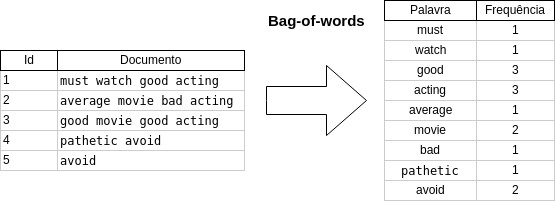
\includegraphics[height=0.2\textheight]{figuras/exemplos/bow-exemplo.png}
  \caption{Exemplo do uso de BoW.}
  \label{fig:exemplo-bow}
\end{figure}

\section{{\it N-gram}}\label{sec:ngram}
N-gramas de textos são amplamente utilizados em tarefas de mineração de texto e processamento de linguagem natural.  N-gram são basicamente uma sequência de termos com o comprimento de $N$ caracteres. 

Usando como exemplo a Figura \ref{fig:exemplo-ngram}, ao utilizar N-gram em um determinado documento, cada termo é dividido em $N$ sequências. Tendo $N=1$ (unigram) cada termo é separado individualmente. Para o $N=2$ (bigram), os termos são divididos de dois em dois e o mesmo serve para o $N=3$. Cada termo criado pelo \textit{N-gram} pode ser representado como uma nova característica, como mostra na Tabela \ref{tab:exemplo-ngram}.  

\begin{figure}[ht]
  \centering
  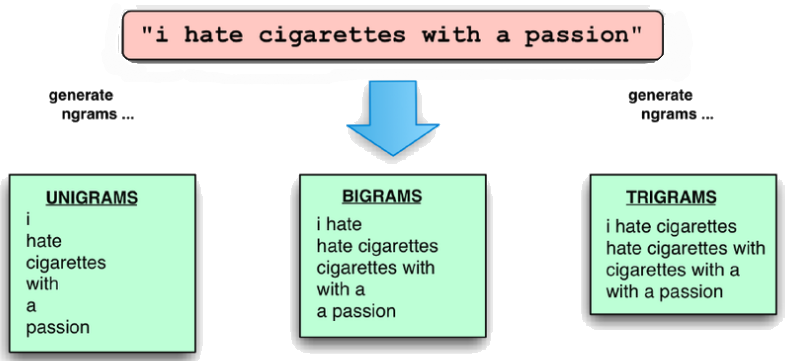
\includegraphics[height=0.3\textheight]{figuras/exemplos/ngram-exemplo.png}
  \caption{Exemplo do uso de N-gram. \cite{exemplongram}}
  \label{fig:exemplo-ngram}
\end{figure}


\begin{table}[h]
\scalebox{0.8}{
\begin{tabular}{c|c|c|c|c|c|c|c|c}
\hline
 {\bf Documento} & \textbf{a} & \textbf{a passion} & \textbf{cigarretes} & 
 \textbf{cigarretes with} & \textbf{cigarretes with a} & 
 \textbf{hate} & \textbf{hate cigarretes} & \textbf{...} \\
 \hline
\textbf{1} & 1 & 1 & 1 & 1 & 1 & 1 & 1 & ... \\
\textbf{2} & 0 & 0 & 1 & 1 & 0 & 0 & 0 & ... \\
\textbf{3} & 1 & 1 & 0 & 0 & 0 & 0 & 0 & ... \\ \hline
\end{tabular}
}
\caption{Exemplo de características utilizando N-gram.}\label{tab:exemplo-ngram}
\end{table}


\section{TF-IDF}\label{sec:tfidf}
O \textit{TF-IDF} tem como objetivo atribuir um peso para as palavras que aparecem com menos frequência nos documentos. Muitas vezes a importância de uma palavra não se dá somente pela sua frequência. 

Documentos maiores, geralmente, são representados por muitos termos. Quando uma grande quantidade de termos é utilizada na representação de documentos, a probabilidade do termo pertencer a um documento é alta e, assim, documentos maiores têm melhores chances de serem relevantes do que documentos menores \cite{tfidf-martins2003metodologia}, como é o caso de \textit{bag-of-words}, visto na Seção \ref{sec:bag-of-words}.

O \textit{term frequency (tf)} é uma métrica que utiliza o número de ocorrências do termo $tj$ no documento $di$. No entanto, quando termos com alta frequência aparecem em todos (ou na maioria) dos documentos da coleção, os mesmos não fornecem informação útil para os atributos nos documentos. Assim, a medida \textit{inverse document frequency (idf)} favorece termos que aparecem em poucos documentos da coleção. As definição do TF e do IDF serão apresentadas a seguir:

\[ tf = \frac{tj}{di} \]
onde $tf$ é o número de vezes que o termo $tj$ ocorre no documento $di$.

\[ idf = log(\frac{d}{t}) \]
onde $t$ é o número de documentos que contém o termo e $d$ é o número total de documentos (\textit{corpus});

\[ tfidf = tf * idf\]
no qual as medidas $tf$ e $idf$ são combinadas.

\section{Stemização}\label{sec:stem}
Na criação da tabela atributo-valor utilizada por algoritmos de Aprendizado de Máquina, cada termo que aparece no documento pode ser mapeado como uma coluna na tabela. Assim, o número de dimensões do conjunto de atributos pode ser grande, gerando  um problema que deve ser minimizado. 

Vários métodos podem ser utilizados a fim de reduzir a quantidade de atributos visando uma melhor representatividade e melhor desempenho do processo de predição. Entre outros, a transformação de cada termo para o radical que o originou, por meio de algoritmos de stemização (\textit{stemming}), é um método amplamente utilizado e difundido, conforme \cite{tfidf-martins2003metodologia}.

Segundo \cite{jivani2011comparative}, a stemização é uma etapa de pré-processamento na mineração de textos e recuperação de informação,  bem como um requisito muito comum de funções de processamento de linguagem natural (PNL). Podemos dizer que o objetivo da stemização é reduzir palavras para uma forma mais básica e comum de escrita. A ideia principal é melhorar o manuseio automático de terminações de palavras, reduzindo as mesmas às suas raízes de palavras. Geralmente, a stemização é feita removendo quaisquer sufixos e prefixos (afixos) anexados nas palavras, dado que o radical de um termo representa um conceito mais amplo do que o termo original. Na Tabela \ref{tab:exemplo-stem} é exemplificada a aplicação da stemização para a redução das variações do radical \textit{quilometr}.

Na stemização, a conversão de formas morfológicas de uma palavra ao seu tronco é feita supondo que cada um é semanticamente relacionado. O radical não precisa ser uma palavra existente no conjunto de atributo-valor, mas todas as suas variantes devem ser mapeadas para este radical. Há dois pontos a serem considerados ao usar o método de stemização:

\begin{itemize}
    \item se as formas morfológicas de uma palavra têm o mesmo significado básico, devem ser mapeadas para o mesmo radical;

    \item palavras que não têm o mesmo significado devem ser mantidas separadamente.
\end{itemize}

Essas duas regras são boas o suficiente, desde que os valores resultantes sejam úteis para a mineração de texto ou PNL. Segundo \cite{jivani2011comparative}, a utilização da stemização é geralmente considerada como um dispositivo de melhoria de revocação (frequência em que um classificador encontra os exemplos de uma classe). Para linguagens com morfologia relativamente simples, a influência da stemização é menor do que para aquelas com morfologia mais complexa.

% exemplo stemização
\begin{table}[h]
    \centering
    % distancia entre a linha e o texto
    {\renewcommand \arraystretch{1.25}
        \begin{tabular}{ l | l }
            \hline  
            \textbf{Palavra} & \textbf{Stem} \\  
            \hline
            quilométricas & quilometr \\  
            quilométricos & quilometr \\  
            quilômetro & quilometr \\  
            quilômetros & quilometr \\  
            \hline
        \end{tabular} 
    }
    \caption{Exemplo de Stemização}\label{tab:exemplo-stem}
\end{table}

Um dos algoritmos de stemização mais conhecidos é o algoritmo de Porter que remove sufixos de termos em inglês \cite{porter2001snowball}.

\section{KNN}\label{sec:knn}
O KNN ({\it K-Nearest-Neighbor}, em português, K-vizinho mais próximo) é um classificador que procura K documentos do conjunto de treinamento que estejam mais próximos deste documento com classificação desconhecida, ou seja, que tenham a menor distância.

Estes $K$ documentos são chamados de K-vizinhos mais próximos. Verifica-se quais são as classes desses K vizinhos e a classe mais frequente será atribuída à classe do documento desconhecido.

\begin{figure}[ht]
  \centering
  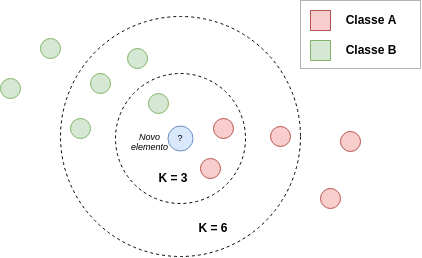
\includegraphics[height=0.2\textheight]{figuras/exemplos/exemplo-knn.png}
  \caption{Exemplo de execução do KNN.}
  \label{fig:exemplo-knn}
\end{figure}

Como pode ser observado no exemplo da Figura \ref{fig:exemplo-knn} a classificação de um novo elemento (em azul) para o $K=3$. Todos os vizinhos mais próximos desse novo elemento são classificados com a classe $A$, portanto, o novo elemento será classificado com a classe $A$. Para o $K=6$, a maioria dos vizinhos mais próximos são de classe $B$, então o novo elemento é classificado como sendo de classe $B$.

A métrica mais comum que calcula a distância é a distância Euclidiana \cite{santos2009variaccoes}. Seja $X=(x_1, x_2,..., x_n)$ e $Y=(y_1, y_2,..., y_n)$ dois pontos de $R^n$, a distância Euclidiana entre X e Y é dada por: 
\[d(x, y) = \sqrt{(x_1-y_1)^2+(x_2-y_2)^2+...+(x_n-y_n)^2}\]

\chapter{Trabalhos Relacionados}\label{cap:trabrel}
%==================================================================
% - Breve explicação
% - Contribuição do artigo
% - Funcionamento básico de método (como chegou na contribuição)
% - Dados usados
% - Tratamento dos dados
% - Features
% - Construção das features
% - Sobre os modelos
% - Conclusão
%==================================================================

% introdução
Neste capítulo serão descritos os principais trabalhos relacionados a este projeto de conclusão de curso.
O capítulo será dividido em duas seções: a primeira delas constituída por alguns trabalhos que identificam discurso de ódio através de modelos de predição, alguns métodos para a criação de novos atributos que ajudam na predição dos dados, bem como os resultados de seus modelos (Seção \ref{sec:trabrel-1}). Na segunda seção é realizada uma análise sobre a extração de meta-atributos (atributos que possuem relação com os atributos originais), utilizando \textit{KNN} para obter informações relevantes de documentos similares, bem como uma análise sobre os seus resultados (Seção \ref{sec:trabrel-2}).

\section{Identificação de discurso de ódio}\label{sec:trabrel-1}

\subsection{Detecção automatizada de discurso de ódio e o problema da linguagem ofensiva}\label{sec:trabrel-1.1}

% objetivo do trabalho
O trabalho de \cite{davidson2017automated} tem por objetivo a classificação em três classes de textos (documentos): discurso de ódio, discurso ofensivo e não ofensivo. O discurso de ódio é definido, conforme \cite{nockleby2000hate}, como qualquer comunicação que deprecie uma pessoa ou um grupo com base em alguma característica como raça, cor, etnia, gênero, orientação sexual, nacionalidade, religião ou outras. Já discurso ofensivo é categorizado, segundo \cite{davidson2017automated}, como documentos que têm linguagem ofensiva mas que não discrimina as pessoas ou um grupo de pessoas.

O discurso de ódio pode ser usado de diferentes maneiras: 
\begin{itemize}
    \item Pode ser enviado diretamente para uma pessoa ou grupo de pessoas;
    \item Pode ser direcionado para ninguém em particular (sarcasmo, ironia);
    \item Em conversas entre pessoas (comentários de redes sociais, fóruns de discussão, sala de bate-papos, etc).
\end{itemize}

%Em muitos trabalhos que tentam classificar um determinado documento como discurso de ódio ou não, 
Neste trabalho é proposta a divisão entre discurso de ódio e discurso ofensivo por alguns motivos. Em muitos casos, textos apresentam palavras ofensivas, mas que de fato não expressam ódio contra outras pessoas, por exemplo, o uso do sarcasmo entre amigos, muitas vezes considerado como brincadeira. Esse tipo de linguagem é comum nas mídias sociais \cite{kwok2013locate}, tornando a tarefa de classificação crucial para qualquer sistema que tente detectar discurso de ódio em documentos.

% como gerou a base
Para a construção dos dados foram utilizadas palavras e frases (\textit{tokens}) de ódio retiradas de um repositório \textit{on-line}\footnote{\url{https://www.hatebase.org/}} de discurso de ódio. Com esse conjunto de palavras e frases, foi feita uma seleção de \textit{tweets} que continham esses \textit{tokens}, resultando em 33.458 de usuários do twitter e 85,4 milhões de documentos (todos em inglês). Desses dados foram selecionados aleatoriamente 25.000 documentos para realização do experimento.

A classificação desses documentos foi realizada por pessoas (garantindo uma classificação mais correta) que tinham que escolher/votar em uma das três categorias que o documento pertencesse: discurso de ódio, discurso ofensivo e não ofensivo. Os classificadores foram instruídos que a presença de uma determinada palavra, embora ofensiva, não indica necessariamente que um documento é discurso de ódio. Cada documento foi classificado três ou mais vezes, sendo enquadrado na categoria que obteve mais votos. Depois dessa classificação manual, resultaram 24.802 documentos rotulados, alguns desconsiderados pela falta de votos.

Apenas 5\% dos documentos foram rotulados como discurso de ódio pela maioria dos classificadores e apenas 1,3\% foram classificados de forma unânime. A maioria dos documentos foi considerada discurso ofensivo (76\% classificados com 2/3 votos, 53\% classificados com 3/3 votos) e o restante foi considerado não ofensivo (16,6\% classificado de 2/3, 11,8\% em 3/3 vezes).

% construção dos atributos
Para a construção dos atributos, cada documento foi formatado em letras minúsculas para evitar divergências. Também foi utilizado o algoritmo de{\it Porter stemmer} para a remoção dos sufixos das palavras e o {\it N-gram} para a construção dos atributos, com os valores de $N={1,2,3}$. A atribuição dos pesos para os atributos foi feita {\it TF-IDF}. (veja na Seção \ref{sec:tfidf}.). Para capturar informações sintáticas dos textos foi usado {\it Part-of-Speech (POS)} juntamente com {\it N-gram} para gerar novos atributos que caracterizam informações da estrutura sintática dos documentos. Para capturar a qualidade de cada documento foi usado o cálculo de {\it Flesch Reading Ease}, que indica se o texto é compreensível para a leitura, onde os valores vão de 0 a 100; quanto maior a pontuação, mais fácil é a leitura. 

Outras características aplicadas no trabalho, levando em consideração os documentos utilizados, foram valores quantitativos extraídos dos textos como a contagem de \textit{hashtags}, menções, \textit{retweets} e \textit{URLs}, bem como recursos para o número de caracteres, palavras e sílabas em cada \textit{tweet}.

% construção do modelo
Para criação do modelo de predição foram testados uma variedade de modelos: regressão Logística, \textit{Naive Bayes}, Árvores de Decisão, Florestas Aleatórias e o \textit{SVM}. Cada modelo foi testado usando validação cruzada de 5 vezes, mantendo 10\% da amostra para avaliação. Os resultados do \cite{davidson2017automated} mostram que Regressão Logística e \textit{SVM} tendem a ter um desempenho significativamente melhor do que outros modelos.

\begin{figure}[ht]
  \centering
  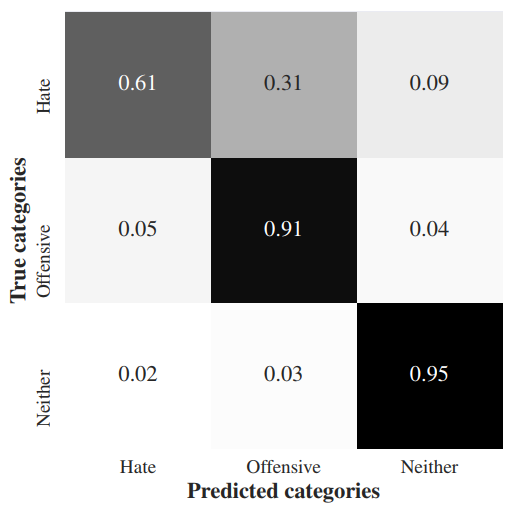
\includegraphics[height=0.4\textheight]{figuras/trab1-confusion-matriz.png}
  \caption{Matriz de confusão dos resultados com \textit{F1-Score} \cite{davidson2017automated}.}
  \label{fig:tb1confmatriz}
\end{figure}

Segundo o artigo, o classificador com melhor desempenho teve uma precisão geral de 91\%, revocação de 90\% e pontuação de F1 de 90\%. No entanto, observando a Figura \ref{fig:tb1confmatriz} percebe-se que quase 40\% dos discursos de ódio são classificados incorretamente: os resultados de precisão e revocação para a classe de ódio são 44\% e 61\%, respectivamente. A maior parte da classificação incorreta ocorre no triângulo superior da matriz, sugerindo que o modelo é favorável a classificar os documentos como menos ódio ou ofensivos do que os codificadores humanos. Um menor número de documentos são classificados como mais ofensivos ou odiosos do que sua verdadeira categoria, aproximadamente 5\% de documentos ofensivos e 2\% de não-ofensivo foram erroneamente classificados como discurso de ódio. 

\subsection{Detecção de Linguagem Abusiva em Conteúdos Online}\label{sec:trabrel-1.2}

% objetivo do trabalho
Em \cite{nobata2016abusive} são utilizados vários métodos de Processamento de Linguagem Natural (PLN) para criação de atributos. Tal trabalho combina algumas características do trabalho apresentado na Seção \ref{sec:trabrel-1.1} e propõe alguns novos atributos para  aprimorar os  resultados. Diversos métodos de PLN foram usados em trabalhos anteriores até então estudados, mas esses recursos nunca foram combinados ou avaliados uns contra os outros para identificar se existe ganho de informação com a combinação. No estudo foi proposto exatamente uma junção de vários métodos para a criação e seleção dos atributos que identificam discurso de ódio em documentos.

No trabalho, a classificação contém as categorias de texto \textit{abusivo} e \textit{não abusivo}. Textos abusivos se referem ao discurso de ódio (comunicação que deprecie uma pessoa ou um grupo de pessoas), ao passo que os não abusivos não contêm discurso de ódio.

% como gerou a base
% Aproximadamente são 215 mil comentários, entre finanças e notícias, 759.402 e 1.390.774 documentos, respectivamente.
Os dados utilizados no trabalho para a detecção de linguagem abusiva são todos de comentários do site do {\it Yahoo}, mais especificamente, comentários pertencentes as categorias de finanças e notícias. Comentários abusivos da categoria de finanças representam 7\% e 16,4\% na categoria de notícias. 

% construção dos atributos
Para à construção dos atributos, foram usadas características que podem ser divididas em quatro classes: \textit{N-grams}, características linguística, características sintáticas e distribuição semântica.
Em características linguísticas, são usadas informações do texto para a criação de atributos, como em alguns exemplos:
\begin{itemize}
    \item Tamanho dos comentários em {\it tokens};
    \item Tamanho médio das palavras;
    \item Número de pontuações do documento;
    \item Quantidade de letras capitalizadas;
    \item Quantidade de palavras desconhecidas do dicionário (em inglês).
\end{itemize}

\newpage
Já as características sintáticas se preocupam em classificar os termos do documento.
Um dos métodos para realizar esse tipo de operação, {\it Part-of-Speech} (PoS), é o processo de marcação de uma palavra em um texto como correspondente a uma parte específica de discurso. A marcação é feita através de {\it tags} que identificam em que parte específica do discurso a palavra se encontra, como por exemplo, marcar palavras que são substantivos, verbos, nomes próprios, etc.

Distribuição semântica é um subcampo do PLN que aprende o significado dos usos das palavras. Alguns métodos que trabalham com características semânticas foram referenciados no artigo. Um exemplo é o método \textit{Word2vec}, que são redes neurais superficiais de duas camadas  treinadas para reconstruir contextos linguísticos de palavras através da coleção de documentos, assim podendo gerar novos atributos.

% construção do modelo
O modelo, foi treinado e testado utilizando o conjunto de dados para ambos os domínios (finanças e notícias). Para cada domínio, foi usado 80\% para treinamento e 20\% para teste. A Figura \ref{fig:tb2resultmodel} mostra a tabela dos resultados de cada domínio quando um modelo treinou com um único tipo de recurso e com todos os recursos combinados. Para ambos os domínios, a combinação de todos os recursos gera o melhor desempenho (79,5\% para finanças e 81,7\% para notícias). As notícias têm uma ligeira vantagem de desempenho, devido ao conjunto de treinamento maior disponível para esse domínio.

\begin{figure}[ht]
  \centering
  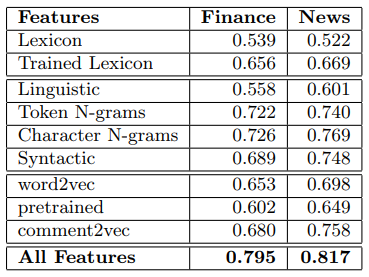
\includegraphics[height=0.3\textheight]{figuras/tabela-modelo-trab2.png}
  \caption{Tabela de resultados para os atributos utilizados do modelo de predição com \textit{F1-Score} \cite{nobata2016abusive}.}
  \label{fig:tb2resultmodel}
\end{figure}


\section{Comentários Ofensivos na Web Brasileira}\label{sec:trabrel-br}
No trabalho \cite{Pelle2017} é apresentado um conjunto de dados com comentários ofensivos (e não ofensivos) coletados na web brasileira. Juntamente com os dados, é apresentado resultados de algoritmos de classificação que servem como base para demais trabalhos futuros.

Os dados foram extraídos de um site brasileiro de notícias, dentre eles foram selecionado 1.250 comentários aleatoriamente. Seguindo o padrão adotado para a classificação dos dados, cada comentário foi anotado por três pessoas com o objetivo de dizer se o comentário é ofensivo ou não.

Foram criadas duas base de dados. A primeira, chamada de {\it OffComBR-2}, possui todos os 1.250 registros (419 classificados como ofensivo) e a classificação atribuída a cada comentário foi determinada por pelo menos duas pessoas. Já a segunda base de dados, {\it OffComBR-3}, possui 1.033 registros (202 ofensivos) e cada comentário foi classificado pelas três pessoas.

Para a classificação dos textos foram criados algumas conjuntos para testes, utilizando métodos PLN, totalizando 24 amostras, 12 para cada base de dados, como podem ser visualizadas na Figura \ref{fig:pelle-statistic}, na qual é possível ver o nome de cada conjunto e o número de características. Segue abaixo os métodos utilizados para formação dos conjuntos:

\begin{itemize}
    \item Redução do Texto: Nesse método, é criado conjuntos de dados com o texto original ({\it original}) e outros com o texto em caixa baixa ({\it lower}).
    \item Tokenização: O texto é dividido em {\it tokens}, onde cada {\it token} é formado por {\it n-grams} e cada {\it unigram} (${1G}$), {\it unigram} e {\it bigram} (${1G+2G}$) e {\it unigram}, {\it bigram} e {\it trigram} (${1G+2G+3G}$) são combinados. Cada {\it token} representa como uma nova característica no conjunto a ser classificado.
    \item Ganho de informação: É selecionado somente características e tem correlação positiva com a classe a ser predita (${FS}$).
\end{itemize}

\begin{figure}[ht]
  \centering
  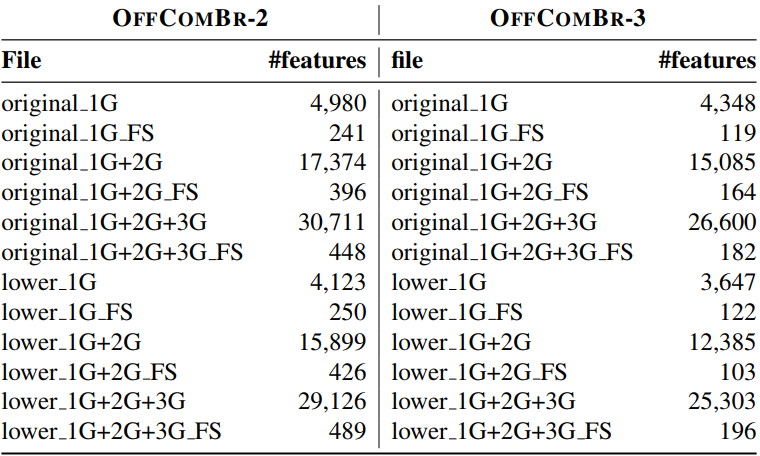
\includegraphics[height=0.3\textheight]{figuras/stats-datasets-offcombr.png}
  \caption{Estatística dos conjuntos de dados \cite{Pelle2017}.}
  \label{fig:pelle-statistic}
\end{figure}

Os algoritmos usado para realizar a classificação do texto foram SVM ({\it Support Vector Machine}) e NB ({\it Naive Bayes}). Como mostra na Figura \ref{fig:pelle-results}, SVM teve um melhor resultado em ambas as base de dados. A base de dados {\it OffComBR-3} teve um melhor resultado, pois a pré-classificação de texto ofensivo está mais definida, onde o texto ofensivo foi classificado pelas três pessoas, ao contrário da {\it OffComBR-2}.

\begin{figure}[ht]
  \centering
  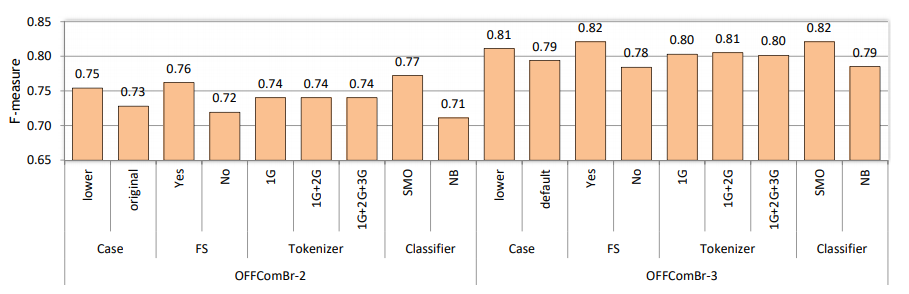
\includegraphics[height=0.2\textheight]{figuras/results-datasets-offcombr.png}
  \caption{Resultados da Classificação dos textos para cada conjunto de características \cite{Pelle2017}.}
  \label{fig:pelle-results}
\end{figure}

\section{Extração de meta-atributos}\label{sec:trabrel-2}

O trabalho \cite{canutoestudo} apresenta um estudo sobre extração de meta-atributos para classificação de textos. Meta-atributos são, em geral, manualmente projetados e extraídos de outros atributos na qual o conjunto de treinamento já é rotulado, e capturam relações fundamentais entre o par \textit{(documento, classe)} ou a tripla \textit{(documento, classe, algoritmo)}. 

Os meta-atributos são capturados usando a  vizinhança de um certo documento de teste a ser classificado utilizando o algoritmo de KNN para identificar os $K$ vizinhos próximos. O trabalho apresenta um estudo comparativo entre utilizar somente meta-atributos, somente os atributos originais da classificação de textos e combinar meta-atributos com os atributos originais.

% meta-atributos
Os meta-atributos baseados em KNN ($M = {mf}$) propostos  contém os vetores de meta-atributos expressos como a concatenação dos sub-vetores descritos a seguir. Cada vetor de atributos $mf$ é definido para um exemplo $xf \in X$ e categoria $cj \in C$ para $j = 1, 2, ... , m$. Segue abaixo os três meta-atributos propostos no artigo:

\begin{itemize}
    \item ${\vec{v}_\vec{x_f}}^{cnt} = [n_j]$:  consiste em um vetor de uma dimensão (tamanho 1) dado pela contagem dos $n_j$ vizinhos (entre os $k$ vizinhos) de $\vec{x_f}$ que são exemplos de treino associados à determinada categoria $c_j$.
    \item ${\vec{v}_\vec{x_f}}^{ncnt} = [\frac{n_j}{n_{max}}]$: consistem em um vetor unidimensional dado pelo número $n_j$ de vizinhos (entre os $k$ vizinhos) de $\vec{x_f}$. O valor de $n_{max}$ corresponde ao número de exemplos associados à classe com o maior número de exemplos dentre os vizinhos mais próximos.
    \item ${\vec{v}_\vec{x_f}}^{qrt} = [\cos{(\vec{x}_{ej}, \vec{x_f})}]$: um vetor de dimensão 5 produzido ao considerar cinco pontos que caracterizam a distribuição de distâncias de $\vec{x_f}$ para seus $j$ vizinhos de dada categoria. As distâncias entre dois vetores $\vec{a}$ e $\vec{b}$ são computadas por similaridade do cosseno, denotada como $\cos{(\vec{a}, \vec{b})}$. Entre todos os pontos de distância entre $\vec{x_f}$ e seus $j$ vizinhos de dada categoria, os cinco pontos selecionados $\cos{(\vec{x}_{1j}, \vec{x_f})}, \cos{(\vec{x}_{2j}, \vec{x_f})}, ... , \cos{(\vec{x}_{5j}, \vec{x_f})}$ correspondem, respectivamente, à menor distância, à
maior distância, à distância média, o quartil inferior (valor que delimita os 25\% dos menores pontos) e o quartil superior (valor que delimita os 25\% dos maiores pontos).
\end{itemize}

Os meta-atributos descritos acima tem uma dimensão de $7$ por categoria. Esse pequeno conjunto de meta-atributos é capaz de capturar informação do conjunto rotulado de três diferentes formas (conforme descrito nos itens acima). A primeira simplesmente conta o número de exemplos rotulados de cada categoria entre os $k$ mais similares exemplos rotulados. A segunda divide o número de vizinhos em cada classe pelo número de vizinhos da classe com maior número de vizinhos, com objetivo de capturar a relação entre a classe escolhida pelo KNN (a classe com maior número de vizinhos) e as outras classes. A última informação fornecida com os meta-atributos propostos é baseada em uma análise das distâncias e distribuição das classes observada na vizinhança do exemplo. Os pontos que caracterizam essas informações são: a menor distância, a maior distância, a mediana, o quartil inferior e o quartil superior.

Os experimentos realizados são em cinco coleções de textos amplamente utilizadas na literatura de classificação automática de texto:

\begin{enumerate}
    \item \textit{4 Universities (4UNI)}. Essa coleção contém páginas da Web coletadas de departamentos de Ciência da Computação de quatro universidades. Existe ao todo 8.277 páginas Web, classificadas em 7 categorias;
    \item \textit{Reuters (REUT)}. Coleção de textos classificados, com artigos de notícias coletados e anotados. Foram considerados 8.184 artigos, classificados em 8 categorias;
    \item \textit{ACM-DL (ACM)}. Um subconjunto da Biblioteca Digital da ACM, com 24.897 documentos contendo artigos relacionados à ciência da computação. Foi considerado apenas o primeiro nível de taxonomia adotado pela ACM, onde cada documento é associado a uma das 11 classes;
    \item \textit{20 Newsgroups (20NG)}. É uma coleção composta de aproximadamente 18.805 documentos de grupo de notícias particionados (aproximadamente) de forma uniforme entre 20 diferentes categorias;
    \item \textit{Spambase (SPAM)}. Uma coleção com diferentes tipos de e-mail. Há um total de 4.601 e-mails classificados como spam ou não-spam;
\end{enumerate}

Os meta-atributos foram avaliados usando duas medidas padrão de classificação de textos: \textit{micro averaged} F1 (MicroF1) que mede a eficácia da classificação sobre todas as decisões, e a \textit{macro averaged} F1 (MacroF1) que mede a eficácia da classificação para cada classe individualmente e obtém a média. Todos os experimentos foram feitos utilizando validação cruzada com 5 partições.

Para a execução dos experimentos e realização da predição dos textos, foi utilizado o algoritmo \textit{SVM}. O tamanho da vizinhança para o algoritmo \textit{KNN} responsável pela geração dos meta-atributos foi definido como sendo \textit{K = 30} (valor tradicionalmente adotado em classificação de texto) para todos os experimentos.

\chapter{Proposta}\label{cap:proposta}

Conforme descrito neste trabalho,métodos de aprendizado de máquina são usados  para identificar conteúdo indevido em textos. Para tais métodos, utilizar boas características (\textit{features}) ajudam a obter melhores resultados durante a classificação.

Identificar discurso de ódio em documentos com a utilização de aprendizado de máquina requer a aplicação de alguns métodos de PLN (apresentados no Capítulo \ref{cap:trabrel} dos Trabalhos Relacionados). O trabalho de \cite{davidson2017automated} e do \cite{nobata2016abusive} (Seção \ref{sec:trabrel-1.2} e  Seção \ref{sec:trabrel-1.1}, respectivamente), utilizam métodos de pré-processamento de textos para criação de suas características, no qual é usado combinações de muitos atributos que ajudam o modelo de predição a ter um melhor desempenho. Já no trabalho de \cite{canutoestudo} (descrito na Seção \ref{sec:trabrel-2}), é proposto a criação de meta-atributos a partir de dados previamente rotulados, onde o objetivo é capturar informações novas e relevantes sobre uma distribuição de dados desconhecida
que relaciona os padrões observados às suas respectivas categorias. 

A proposta deste trabalho é extrair novas características a partir de meta-atributos gerados através de informações retirados vizinhança de cada documento, inspirado no trabalho de \cite{canutoestudo}, os meta-atributos são encontrados através do algoritmo de classificação KNN, descrito na Seção \ref{sec:knn}. A base de dados a ser utilizada é a mesma abordada por \cite{Pelle2017} juntamente com os seus conjuntos para teste, apresentado na Seção \ref{sec:proposta-base-dados}.

\section{Método Proposto}
Esta seção tem por objetivo descrever como funciona o método proposto aplicado neste trabalho. 

Para aplicação do método, inicialmente é usado o algoritmo de classificação KNN para encontrar a vizinhança mais próxima dos documentos previamente rotulados. A distancia usada para determinar a proximidade dos vizinhos ao documento, é definida pela similaridade do cosseno. 

Com as informações da vizinhança para cada documento, é feita a criação de novas características a partir das mesmas. A proposta das novas características é capturar informação do conjunto já rotulado de três diferentes formas:

\begin{enumerate}
    \item Contagem de exemplos rotulados, da mesma maneira que fez o método kNN;
    \item Capturar a relação entre a classe escolhida pelo kNN (a classe com maior número de vizinhos) com a outra classes;
    \item Análise da distribuição das distâncias para cada classe.
\end{enumerate}

% \begin{itemize}
%     \item {\bf Menor distância}: Dentre todos os vizinhos, foi escolhido o mais próximo, e com a menor distância é definida a característica.  
%     \item {\bf Maior distância}: De todos os vizinhos é escolhido o mais distante e atribuindo a maior distancia como uma característica.
%     \item {\bf Média distância}: Característica criada a partir da média de todas as distâncias dos vizinhos.
%     \item {\bf Contagem de vizinhos}: É feito uma contagem dos vizinhos de determinada classe.
%     \item {\bf Razão entre as classes}: Para tal, basta dividir o número de vizinhos em cada classe pelo número de vizinhos da classe com maior número de vizinhos, com objetivo de capturar a relação entre a classe escolhida pelo kNN e as outras classes.
%     \item {\bf Quartil inferior}: valor que delimita os 25\% das menores distâncias.
%     \item {\bf Quartil superior}: valor que delimita os 25\% das maiores distâncias.
% \end{itemize}

\chapter{Experimentos e Resultados}

Neste capítulo, serão apresentados os resultados obtidos para cada experimento. Serão detalhados os algoritmos que foram utilizados para a classificação dos dados, conforme descritos na proposta deste trabalho, Seção \ref{cap:proposta}. A Seção \ref{sec:proposta-base-dados} tem como objetivo mostrar a base de dados que foi utilizada para realização dos teste e também a descrição de cada experimento proposto. Já na Seção \ref{sec:proposta-metricas} e \ref{sec:proposta-experimentos} são apresentadas as métricas utilizadas para cada experimento e os seus resultados.  

Vale ressaltar, os experimentos e resultados foram construídos e avaliados com ferramentas diferentes ao trabalho de \cite{Pelle2017}. Para o trabalho relacionado, os resultados foram obtidos pela ferramenta {\it Weka}, neste trabalho, foi utilizado outros recursos descritos na Seção \ref{sec:codigo-fonte}, e parâmetros obrigatórios de algoritmos foram os mesmos utilizados no {\it Weka}. É notável uma diferença na quantidade de características e em alguns resultados obtidos, porém, ambas não comprometem o resultado obtido. 

\section{Base de Dados}\label{sec:proposta-base-dados}
A base de dados apresentada no trabalho relacionado \cite{Pelle2017}, Seção \ref{sec:trabrel-br}, e que pode ser obtida por {\it download} \footnote{\url{https://github.com/rogersdepelle/OffComBR}} foi utilizada para a realização dos experimentos.

Como visto anteriormente na Seção \ref{sec:trabrel-br}, a base de dados é composta por duas partes denominadas {\it OffComBR-2} e {\it OffComBR-3}. As duas contêm os textos (comentários da web) juntamente com o rótulo de classificação, na qual indica se o texto representa discurso de ódio (classificação positiva) ou não. Na primeira parte, composta por 1.250 comentários, 419 destes são considerados discurso de ódio, representando aproximadamente de 33,5\% e cada rótulo foi classificado por pelo menos duas pessoas. Já na segunda, são 1.033 comentários, 202 dos mesmos são considerados discurso de ódio, que representa aproximadamente 19,55\% dos dados e a classificação foi atribuída por três pessoas. Ambos os dados podem ser visto na Tabela \ref{tab:proposta-base-dados}.

\begin{table}[h]
    \centering
    % distancia entre a linha e o texto
    {\renewcommand \arraystretch{1.25}
        \begin{tabular}{ c c c }
            \hline
            {\bf Base de Dados} & {\bf Total de Comentários} & {\bf Classificação Positiva} \\
            \hline
            
            {\it OffComBR-2} & 1.250 & 419 \\
            {\it OffComBR-3} & 1.033 & 202 \\  
            \hline
        \end{tabular} 
    }
    \caption{Estatística das Bases de Dados.}\label{tab:proposta-base-dados}
\end{table}

Para a aplicação do método, foram criados alguns conjuntos de experimentos, os mesmos propostos em \cite{Pelle2017}. Para cada experimento foi criado determinadas características utilizando alguns métodos de PLN. Como é apresentado na Tabela \ref{tab:proposta-base-dados-experimentos}, experimentos com o prefixo {\it original} foram mantidos o texto com a forma original do comentário. Já experimentos com prefixo {\it lower}, o texto foi transformado em caixa baixa, diminuindo assim a dimensionalidade das características. Alguns experimentos possuem combinações de {\it N-gram}, conforme indicado na Tabela \ref{tab:proposta-base-dados-experimentos}, experimentos que usam {\it 1-gram}, {\it 2-gram} ou {\it 3-gram} estão marcados como {\it Sim}. A coluna {\it FS} indica se o experimento possui somente as melhores características utilizando o ganho de informação. {\it TC2} e {\it TC3} mostram o total de características para cada experimento nas base de dados {\it OffComBR-2} e {\it OffComBR-3} respectivamente.     

\begin{table}[h]
    \centering
    % distancia entre a linha e o texto
    {\renewcommand \arraystretch{1.25}
        \begin{tabular}{ l c c c c c c }
            \hline
            {\bf Experimento} & {\it \bf 1-gram } & {\it \bf 2-gram } & {\it \bf 3-gram } &
            {\bf MC } & {\bf TC2 } & {\bf TC3 } \\  
            \hline
            
            {\it original\_1G} & Sim & Não & Não & Não & 4.979 & 4.347 \\
            {\it original\_1G\_FS} & Sim & Não & Não & Sim & 261 & 148 \\
            {\it original\_1G\_2G} & Sim & Sim & Não & Não & 17.373 & 15.084 \\
            {\it original\_1G\_2G\_FS} & Sim & Sim & Não & Sim & 263 & 146 \\
            {\it original\_1G\_2G\_3G} & Sim & Sim & Sim & Não & 30.710 & 26.599 \\
            {\it original\_1G\_2G\_3G\_FS} & Sim &  Sim & Sim & Sim & 260 & 151 \\
            {\it lower\_1G} & Sim &  Não & Não & Não & 4.122 & 3.646 \\
            {\it lower\_1G\_FS} & Sim &  Não & Não & Sim & 259 & 144 \\
            {\it lower\_1G\_2G} & Sim &  Sim & Não & Não & 15.898 & 13.881 \\
            {\it lower\_1G\_2G\_FS} & Sim &  Sim & Não & Sim & 263 & 142 \\
            {\it lower\_1G\_2G\_3G} & Sim &  Sim & Sim & Não & 29.125 & 25.302 \\
            {\it lower\_1G\_2G\_3G\_FS} & Sim &  Sim & Sim & Sim & 268 & 146 \\
            \hline
        \end{tabular} 
    }
    \caption{Experimentos e suas Característica referente ao trabalho \cite{Pelle2017}}\label{tab:proposta-base-dados-experimentos}
\end{table}

\section{Métricas}\label{sec:proposta-metricas}
Para avaliar a eficácia do método proposto foi utilizado a mesma abordagem do trabalho \cite{Pelle2017}. O métrica avaliada para os experimentos foi {\it f-score}, no qual representa a média harmônica entre precisão e revocação, levando sempre em consideração o peso das classes ({\it f1-weighted}). Para obter uma média mais cofiável dos experimentos, foi usado validação cruzada de dez vezes em cada conjunto de testes e feita a média do {\it f-score} de todas as execuções. 

Para validar as comparações entre os métodos, foi utilizado o teste {\it Student’s T-Test} (t-test) na métrica {\it f-score}. Esse teste é feito sobre dois conjuntos de dados e o seu resultado é um número, entre 0 e 1, que mede a confiança de uma afirmação. Neste trabalho, as afirmações que passam por validação são os resultados do trabalho \cite{Pelle2017} e da proposta deste trabalho. Caso o resultado do {\it t-test} for $\alpha > 0,05$, pode-se afirmar que uma proposta foi melhor ou pior que a outra em um determinado aspecto.

\section{Execução dos Experimentos}\label{sec:proposta-experimentos}

Foram conduzidos experimentos para avaliar a eficácia e o poder discriminativo dos meta-atributos
descritos anteriormente, bem como dos atributos textuais originais. Esses atributos originais serão referenciados nas tabelas como {\it Pelle, 2017}. O grupo dos meta-atributos, método proposto neste trabalho, serão denominados como {\it LIMA}.

Para os experimentos, foram executados dois algoritmos de classificação, o SVM, com os hiper parâmetros sendo: $kernel=linear$ e $C=1.0$. NB foi utilizado com os parâmetros originais do classificador. Cada teste foi executado com validação cruzada de dez vezes. 

A seguir serão apresentados os resultados das execuções em ambas as base de dados, Tabelas \ref{tab:resultados-experimentos-br2} e \ref{tab:resultados-experimentos-br3}. As tabelas mostram os resultados das execuções dos algoritmos de classificação SVM e NB e juntamente com o desvio padrão e a indicação de ganho estatístico de cada média. 

Na base de dados {\it OffComBr-2}, após aplicar o método e suas execuções, apresentados na Tabela \ref{tab:resultados-experimentos-br2}, pode-se perceber  em poucos casos que, a média das execuções entre {\it Pelle, 2017} e a combinação de {\it Pelle, 2017 + LIMA} obteve um resultado maior com o classificador SVM, como a dos experimentos {\it original\_1G\_FS}, {\it original\_1G\_2G\_FS}, {\it lower\_1G\_FS}, {\it lower\_1G\_2G\_FS} e {\it lower\_1G\_2G\_3G\_FS}. Na execução dos experimentos {\it LIMA} com o classificador SVM, todos os resultados foram abaixo ao de {\it Pelle, 2017}. Já o algoritmo de NB chegou em resultados mais próximos ao de {\it Pelle, 2017}.

\begin{table}[h]
\renewcommand \arraystretch{1.25}
\scalebox{0.675}{
\begin{tabular}{l|cccc|cccc|cccc}
\hline
& \multicolumn{4}{c|}{\it \textbf{Pelle, 2017}} & \multicolumn{4}{c|}{\it \textbf{LIMA}} & \multicolumn{4}{c}{\it \textbf{Pelle, 2017 + LIMA}} \\ \hline
\multicolumn{1}{c|}{\textbf{Experimento}} & \multicolumn{1}{c}{\textbf{SVM}} & \multicolumn{1}{c}{\textbf{STD}} & \multicolumn{1}{c}{\textbf{NB}} & \multicolumn{1}{c|}{\textbf{STD}} & \multicolumn{1}{c}{\textbf{SVM}} & \multicolumn{1}{c}{\textbf{STD}} & \multicolumn{1}{c}{\textbf{NB}} & \multicolumn{1}{c|}{\textbf{STD}} & \multicolumn{1}{c}{\textbf{SVM}} & \multicolumn{1}{c}{\textbf{STD}} & \multicolumn{1}{c}{\textbf{NB}} & \multicolumn{1}{c}{\textbf{STD}} \\ \hline
\textit{original\_1G} & 67,12\% & 0,05 & 64,20\% & 0,05 & 61,59\% & 0,04 & 67,00\% & 0,04 & 67,77\% & 0,06 & 64,20\% & 0,05 \\ 
\textit{original\_1G\_FS} & 70,81\% & 0,06 & 65,63\% & 0,03 & 64,14\% & 0,05 & 66,77\% & 0,05 & 72,46\% & 0,05 & 66,14\% & 0,04 \\ 
\textit{original\_1G\_2G} & 66,47\% & 0,05 & 65,81\% & 0,04 & 62,09\% & 0,05 & 68,18\% & 0,04 & 66,81\% & 0,07 & 65,81\% & 0,04 \\
\textit{original\_1G\_2G\_FS} & 70,05\% & 0,06 & 64,15\% & 0,03 & 63,08\% & 0,03 & 64,37\% & 0,05 & 71,23\% $\uparrow$ & 0,05 & 65,83\% & 0,03 \\
\textit{original\_1G\_2G\_3G} & 67,67\% & 0,06 & 65,98\% & 0,04 & 61,71\% & 0,05 & 68,32\% & 0,04 & 66,91\% & 0,05 & 65,98\% & 0,04 \\
\textit{original\_1G\_2G\_3G\_FS} & 70,79\% & 0,06 & 66,90\% & 0,04 & 62,07\% & 0,04 & 64,73\% & 0,06 & 70,82\% & 0,05 & 66,54\% & 0,04 \\
\textit{lower\_1G} & 71,50\% & 0,06 & 65,47\% & 0,05 & 66,20\% & 0,06 & 67,19\% & 0,06 & 71,43\% & 0,05 & 65,47\% & 0,05 \\
\textit{lower\_1G\_FS} & 68,66\% & 0,06 & 45,80\% & 0,08 & 64,57\% & 0,05 & 67,57\% & 0,05 & 72,19\% $\uparrow$ & 0,05 & 47,02\% & 0,10 \\
\textit{lower\_1G\_2G} & 70,49\% & 0,06 & 67,19\% & 0,05 & 67,24\% & 0,05 & 68,53\% & 0,06 & 70,67\% & 0,05 & 67,19\% & 0,05 \\
\textit{lower\_1G\_2G\_FS} & 69,58\% & 0,06 & 63,30\% & 0,05 & 65,29\% & 0,04 & 65,55\% & 0,05 & 72,46\% & 0,04 & 46,50\% & 0,09 \\
\textit{lower\_1G\_2G\_3G} & 69,15\% & 0,06 & 67,57\% & 0,05 & 67,07\% & 0,05 & 69,23\% & 0,06 & 70,99\% & 0,05 & 67,57\% & 0,05 \\
\textit{lower\_1G\_2G\_3G\_FS} & 66,95\% & 0,05 & 41,18\% & 0,11 & 67,94\% & 0,04 & 67,22\% & 0,04 & 72,11\% $\uparrow$ & 0,05 & 43,20\% & 0,10 \\ \hline
\end{tabular}
}
\caption{Experimentos com a base de dados {\it OffComBR-2}.}\label{tab:resultados-experimentos-br2}
\end{table}

Na Tabela \ref{tab:resultados-experimentos-br3}, são apresentados os resultados das execuções com a base de dados {\it OffComBR-3}. Destaca-se que todos os ganhos são maiores pelo fato de que a classificação dos comentários são mais precisos que a da base de dados {\it OffComBR-2}. Ao comparada com os resultados da Tabela \ref{tab:resultados-experimentos-br2}, esses experimentos tiveram ganhos semelhantes. Os experimentos {\it original\_1G\_2G\_3G\_FS}, {\it lower\_1G\_FS}, {\it lower\_1G\_2G\_FS} e {\it lower\_1G\_2G\_3G\_FS}, tiveram uma média maior com a combinação de {\it Pelle, 2017 + LIMA} utilizando o classificador SVM. Com NB, somente o experimento {\it lower\_1G\_FS} obteve melhor resultado. Resultados somente com o método LIMA foram semelhantes ao de {\it Pelle, 2017} com o classificador SVM e inferiores utilizando NB.

\begin{table}[h]
\renewcommand \arraystretch{1.25}
\scalebox{0.673}{
    \begin{tabular}{l|cccc|cccc|cccc}
    \hline
\multicolumn{1}{c|}{} & \multicolumn{4}{c|}{\textit{\textbf{Pelle, 2017}}} & \multicolumn{4}{c|}{\textit{\textbf{LIMA}}} & \multicolumn{4}{c}{\textit{\textbf{Pelle, 2017 + LIMA}}} \\ \hline
\textbf{Experimento} & \textbf{SVM} & \textbf{STD} & \textbf{NB} & \textbf{STD} & \textbf{SVM} & \textbf{STD} & \textbf{NB} & \textbf{STD} & \textbf{SVM} & \textbf{STD} & \textbf{NB} & \textbf{STD} \\ \hline
\textit{original\_1G} & 78,16\% & 0,03 & 77,82\% & 0,07 & 71,73\% & 0,00 & 73,73\% & 0,11 & 78,67\% & 0,04 & 77,82\% & 0,07 \\ 
\textit{original\_1G\_FS} & 80,61\% & 0,03 & 81,07\% & 0,02 & 78,78\% & 0,04 & 77,80\% & 0,04 & 81,42\% & 0,04 & 79,97\% & 0,03 \\ 
\textit{original\_1G\_2G} & 78,02\% & 0,03 & 77,69\% & 0,05 & 71,73\% & 0,00 & 76,67\% & 0,03 & 77,86\% & 0,04 & 77,69\% & 0,05 \\ 
\textit{original\_1G\_2G\_FS} & 79,29\% & 0,02 & 81,14\% & 0,03 & 79,52\% & 0,04 & 77,22\% & 0,04 & 81,71\% & 0,04 & 80,38\% & 0,03 \\ 
\textit{original\_1G\_2G\_3G} & 77,25\% & 0,03 & 77,46\% & 0,05 & 71,95\% & 0,01 & 76,21\% & 0,03 & 77,44\% & 0,05 & 77,46\% & 0,05 \\ 
\textit{original\_1G\_2G\_3G\_FS} & 80,19\% & 0,02 & 78,67\% & 0,03 & 80,49\% & 0,04 & 69,69\% & 0,06 & 82,63\% $\uparrow$ & 0,03 & 79,04\% & 0,03 \\ 
\textit{lower\_1G} & 77,47\% & 0,02 & 76,90\% & 0,07 & 71,73\% & 0,00 & 77,10\% & 0,04 & 77,11\% & 0,03 & 76,90\% & 0,07 \\ 
\textit{lower\_1G\_FS} & 78,86\% & 0,03 & 78,56\% & 0,05 & 81,46\% & 0,04 & 70,09\% & 0,05 & 81,90\% $\uparrow$ & 0,04 & 80,72\% $\uparrow$ & 0,04 \\ 
\textit{lower\_1G\_2G} & 77,62\% & 0,04 & 76,69\% & 0,04 & 71,73\% & 0,00 & 77,26\% & 0,03 & 78,12\% & 0,04 & 76,69\% & 0,04 \\
\textit{lower\_1G\_2G\_FS} & 79,91\% & 0,03 & 78,96\% & 0,05 & 78,16\% & 0,04 & 74,17\% & 0,07 & 82,30\% $\uparrow$ & 0,04 & 77,59\% & 0,05 \\
\textit{lower\_1G\_2G\_3G} & 77,23\% & 0,02 & 76,70\% & 0,04 & 72,12\% & 0,01 & 76,17\% & 0,04 & 77,91\% & 0,04 & 76,70\% & 0,04 \\
\textit{lower\_1G\_2G\_3G\_FS} & 80,36\% & 0,02 & 77,53\% & 0,03 & 82,24\% & 0,04 & 73,10\% & 0,05 & 84,57\% $\uparrow$ & 0,03 & 78,51\% & 0,05 \\ \hline
\end{tabular}
    }
    \caption{Experimentos com a base de dados {\it OffComBR-3}.}\label{tab:resultados-experimentos-br3}
\end{table}

Os resultados que foram considerados como maiores, foi feito o {\it t-test}, assim considerando que os resultados obtiveram um ganho estatístico de 95\% em cima das amostras executadas.


[explicar a média geral dos métodos]

\section{Discussão sobre os resultados}

\section{Código-Fonte}\label{sec:codigo-fonte}
Esta seção apresenta as ferramentas e bibliotecas que foram utilizadas no desenvolvimento do código fonte.
Todas as etapas do processo foram codificadas utilizando a linguagem de programação Python. Para trabalhar com os algoritmos de classificação foi utilizado a biblioteca {\bf scikit-learn}\footnote{\url{https://scikit-learn.org/stable/}}. Esta, possui uma grande quantidade de ferramentas para algoritmos de aprendizado de maquina, além de possuir todas as ferramentas necessárias para fazer a leitura dos arquivos da base de dados. Para realizar o pré-processamento do texto foi utilizado a biblioteca \textbf{nltk}\footnote{\url{https://www.nltk.org/}} ({\it Natural Language Toolkit}).

Todos os códigos das ferramentas utilizadas para os testes estão disponível publicamente.\footnote{\url{https://gitlab.com/cleiton-limapin/tcc-final}}

\chapter{Conclusão}\label{cap:conclusao}
Os experimentos que obtiveram ganho são os que possuem características relevantes utilizando o ganho de informação ({\it *\_FS}). Investigando os mesmos, verificou-se algumas informações semelhantes entre os mesmos: 

\begin{itemize}
    \item As novas características utilizando meta-atributos, todas estavam presentes nos experimentos que utilizam ganho de informação;
    \item Palavras consideradas "palavrões"~ são fortes indicativos de que um comentário pode ser um discurso de ódio;
    \item A letra "a"~ é uma das características mais relevantes.
\end{itemize}
% \chapter{Metodologia}\label{cap:metodologia}
Após a definição da área de pesquisa, o primeiro passo foi a realização de uma busca pelos trabalhos relacionados a mesma. Para isso, foi utilizada a plataforma \textit{Google Scholar}, tendo como entrada os seguintes termos para realizar a busca: {\it "hate speech", "hate speech machine learning", "sentiment social media", "text classification", "text classification feature extraction".} A partir dos resultados obtidos com a busca, os principais trabalhos relacionados ao tema foram selecionados de acordo com a sua relevância (semelhança do tema com o título, quantidade de citações e local de publicação).

Por meio de uma primeira análise dos trabalhos encontrados, duas recentes abordagens foram selecionados, sendo eles: \cite{davidson2017automated} e \cite{nobata2016abusive}, ambas representam trabalhos relevantes na criação de um modelo de predição para identificar discurso de ódio em documentos extraídos da \textit{web}. Já o trabalho  \cite{canutoestudo}, propõe a criação de características, que será utilizada por este projeto. 

A partir da leitura desses trabalhos, observou-se que ambos usam abordagens diferentes para a extração de características levando em conta o contexto em que cada trabalho utilizou para a classificação dos textos. Dessa forma, após a realização do estudo inicial, foi definido como tema deste trabalho, uma proposta para extração de atributos para identificação de textos ofensivos. 

O trabalho está dividido em algumas etapas que determinam o desenvolvimento do mesmo, a fim de se realizar os objetivos que foram definidos. As etapas foram distribuídas da seguinte forma:

\begin{itemize}
    \item \textbf{Etapa 1:} Pesquisa bibliográfica;
    \item \textbf{Etapa 2:} Definição de uma base de dados onde serão aplicados os métodos de extração de características para a realização do trabalho;
    \item \textbf{Etapa 3:} Definição dos métodos que serão utilizado no trabalho para a extração das características;
    \item \textbf{Etapa 4:} Relacionar métodos supervisionados de aprendizagem de máquina para classificar os textos da base de dados;
    \item \textbf{Etapa 5:} Definir métricas para comparar os resultados obtidos com trabalhos relacionados;
    \item \textbf{Etapa 6:} Definir uma forma de apresentar os resultados obtidos pelos experimentos. Avaliar e apresentar os resultados obtidos.
\end{itemize}

% etapa 1
Na \textbf{etapa 1} é retomada a pesquisa bibliográfica do trabalho, que teve início no mês de março de 2018. Compreender os métodos usados para a extração de características é de grande importância, tendo em vista que outros métodos de PLN não citados neste trabalho podem ser incluídos na pesquisa. 

% etapa 2
Durante a \textbf{etapa 2}, foi definida um conjunto de dados já existente para a realização da monografia.
O trabalho \cite{davidson2017automated} possui uma base já rotulada com dados do \textit{twitter}. A classificação é feita em três categorias, descrito na Seção \ref{sec:trabrel-1.1}. 

Já o trabalho \cite{nobata2016abusive} utiliza uma base de dados pública proposta pelo artigo, onde possui vários comentários retirados da \textit{web}. A base é rotulada com duas categorias, o conteúdo do documento pode ser abusivo ou não-abusivo, também visto anteriormente na Seção \ref{sec:trabrel-1.2}. 

Outra base de dados que pode ser utilizado é referente ao trabalho \cite{Pelle2017}, são comentários em língua portuguesa extraídos de um site de notícias, são aproximadamente 1000 documentos previamente classificados, com o intuito de identificar textos ofensivos. A classificação do mesmo diz se o documento é ofensivo ou não-ofensivo.

% etapa 3
A \textbf{etapa 3} é destinada para a definição de quais métodos serão utilizados na pesquisa. Alguns métodos foram apresentados no capítulo \ref{cap:fundamentacaoteorica}. Novos métodos podem ser propostos com a realização da etapa 1. A combinação de métodos como apresentado no trabalho \cite{nobata2016abusive} ou a exclusão de atributos não relevantes para o modelo é uma das opções a serem abordadas.

No trabalho \cite{canutoestudo} é proposto a criação de meta-atributos para a classificação de texto, anteriormente explicado na Seção \ref{sec:trabrel-2}. Neste trabalho pretende-se aplicar tais meta-atributos como um meio  melhorar a qualidade da classificação dos documentos. De acordo com a pesquisa bibliográfica realizada, nenhum trabalho aborda esse tipo de característica.

% etapa 4
A escolha dos algoritmos de aprendizado de máquina supervisionado que serão utilizados para a predição dos dados se dará na \textbf{etapa 4}. Os trabalhos relacionado, vistos na Seção \ref{cap:trabrel}, por exemplo, utilizaram o algoritmo \textit{SVM} para avaliação dos modelos. Nessa etapa será criado outros modelos com algoritmos diferentes de classificação.

% etapa 5
Durante o processo de criação de um modelo de aprendizagem de máquina é preciso medir a qualidade dele de acordo com o objetivo à ser alcançado. Existem funções matemáticas que ajudam a avaliar a capacidade de erro e acerto dos modelos de classificação, elas são chamadas de métricas e serão implementadas na \textbf{etapa 5}, como a Precisão Geral (acurácia), precisão, revocação e \textit{F1 Score} \cite{tfidf-martins2003metodologia}.

% etapa 6
Por fim, a \textbf{etapa 6} consiste em definir a forma com que os resultados serão apresentados. Para isso, as opções de gráficos e tabelas exibindo o comportamento e os valores obtidos pela execução dos experimentos será utilizada.
% \chapter{Cronograma}\label{cap:cronograma}
O cronograma de realização das etapas deste trabalho, vistas no capítulo \ref{cap:metodologia}, está organizado segundo a tabela a seguir. %Cada célula representa uma quinzena do mês da sua referida coluna:

% \begin{table}[h!]
%     \centering
%     \begin{tabular}{|l|l|l|l|l|l|l|l|l|l|l|l|l|}
%     \hline
%     \textbf{Atividade} & 
%     \multicolumn{2}{l|}{\textbf{Jul}} & 
%     \multicolumn{2}{l|}{\textbf{Ago}} & 
%     \multicolumn{2}{l|}{\textbf{Set}} & 
%     \multicolumn{2}{l|}{\textbf{Out}} &
%     \multicolumn{2}{l|}{\textbf{Nov}} & 
%     \multicolumn{2}{l|}{\textbf{Dez}} \\ \hline \hline
%     \textbf{Etapa 1} & x & x & & & & & & & & & & \\ \hline
%     \textbf{Etapa 2} & & x & x & & & & & & & & & \\ \hline
%     \textbf{Etapa 3} & & & x & x & x & & & & & & & \\ \hline
%     \textbf{Etapa 4} & & & & x & x & & & & & & & \\ \hline
%     \textbf{Etapa 5} & & & & & x & x & x & x & & & & \\ \hline
%     \textbf{Etapa 6} & & & & & & & x & x & x & & & \\ \hline
%     Escrita da Monografia & & & & x & x & x & x & x & x & x & x & \\ \hline
%     \end{tabular}
%     \caption{Cronograma de atividades.}
%     \label{my-label}
% \end{table}

\begin{table}[h!]
 \centering
% distancia entre a linha e o texto
 {\renewcommand\arraystretch{1.25}
 \begin{tabular}{ l l l l l l l l l l l }
  \cline{1-1}\cline{2-2}\cline{3-3}\cline{4-4}\cline{5-5}\cline{6-6}\cline{7-7}\cline{8-8}\cline{9-9}\cline{10-10}\cline{11-11}  
    \multicolumn{1}{|p{4cm}|}{\textbf{Atividade} \centering } &
    \multicolumn{1}{p{0.733cm}|}{\textbf{Mar} 2018 \centering } &
    \multicolumn{1}{p{0.733cm}|}{\textbf{Abr} 2018 \centering } &
    \multicolumn{1}{p{0.733cm}|}{\textbf{Mai} 2018 \centering } &
    \multicolumn{1}{p{0.733cm}|}{\textbf{Jun} 2018 \centering } &
    \multicolumn{1}{p{0.733cm}|}{\textbf{Jul} 2018 \centering } &
    \multicolumn{1}{p{0.733cm}|}{\textbf{Ago} 2018 \centering } &
    \multicolumn{1}{p{0.733cm}|}{\textbf{Set} 2018 \centering } &
    \multicolumn{1}{p{0.733cm}|}{\textbf{Out} 2018 \centering } &
    \multicolumn{1}{p{0.733cm}|}{\textbf{Nov} 2018 \centering } &
    \multicolumn{1}{p{0.733cm}|}{\textbf{Dez} 2018 \centering }
  \\  
  \cline{1-1}\cline{2-2}\cline{3-3}\cline{4-4}\cline{5-5}\cline{6-6}\cline{7-7}\cline{8-8}\cline{9-9}\cline{10-10}\cline{11-11}  
    \multicolumn{1}{|p{4cm}|}{\textbf{Etapa 1}} &
    \multicolumn{1}{p{0.733cm}|}{x \centering } &
    \multicolumn{1}{p{0.733cm}|}{x \centering } &
    \multicolumn{1}{p{0.733cm}|}{x \centering } &
    \multicolumn{1}{p{0.733cm}|}{x \centering } &
    \multicolumn{1}{p{0.733cm}|}{x \centering } &
    \multicolumn{1}{p{0.733cm}|}{  \centering } &
    \multicolumn{1}{p{0.733cm}|}{  \centering } &
    \multicolumn{1}{p{0.733cm}|}{  \centering } &
    \multicolumn{1}{p{0.733cm}|}{  \centering } &
    \multicolumn{1}{p{0.733cm}|}{  \centering }
  \\  
  \cline{1-1}\cline{2-2}\cline{3-3}\cline{4-4}\cline{5-5}\cline{6-6}\cline{7-7}\cline{8-8}\cline{9-9}\cline{10-10}\cline{11-11}  
    \multicolumn{1}{|p{4cm}|}{\textbf{Etapa 2}} &
    \multicolumn{1}{p{0.733cm}|}{  \centering } &
    \multicolumn{1}{p{0.733cm}|}{  \centering } &
    \multicolumn{1}{p{0.733cm}|}{  \centering } &
    \multicolumn{1}{p{0.733cm}|}{  \centering } &
    \multicolumn{1}{p{0.733cm}|}{x \centering } &
    \multicolumn{1}{p{0.733cm}|}{x \centering } &
    \multicolumn{1}{p{0.733cm}|}{  \centering } &
    \multicolumn{1}{p{0.733cm}|}{  \centering } &
    \multicolumn{1}{p{0.733cm}|}{  \centering } &
    \multicolumn{1}{p{0.733cm}|}{  \centering }
  \\  
  \cline{1-1}\cline{2-2}\cline{3-3}\cline{4-4}\cline{5-5}\cline{6-6}\cline{7-7}\cline{8-8}\cline{9-9}\cline{10-10}\cline{11-11}  
    \multicolumn{1}{|p{4cm}|}{\textbf{Etapa 3}} &
    \multicolumn{1}{p{0.733cm}|}{  \centering } &
    \multicolumn{1}{p{0.733cm}|}{  \centering } &
    \multicolumn{1}{p{0.733cm}|}{  \centering } &
    \multicolumn{1}{p{0.733cm}|}{  \centering } &
    \multicolumn{1}{p{0.733cm}|}{x \centering } &
    \multicolumn{1}{p{0.733cm}|}{x \centering } &
    \multicolumn{1}{p{0.733cm}|}{  \centering } &
    \multicolumn{1}{p{0.733cm}|}{  \centering } &
    \multicolumn{1}{p{0.733cm}|}{  \centering } &
    \multicolumn{1}{p{0.733cm}|}{  \centering }
  \\  
  \cline{1-1}\cline{2-2}\cline{3-3}\cline{4-4}\cline{5-5}\cline{6-6}\cline{7-7}\cline{8-8}\cline{9-9}\cline{10-10}\cline{11-11}  
    \multicolumn{1}{|p{4cm}|}{\textbf{Etapa 4}} &
    \multicolumn{1}{p{0.733cm}|}{  \centering } &
    \multicolumn{1}{p{0.733cm}|}{  \centering } &
    \multicolumn{1}{p{0.733cm}|}{  \centering } &
    \multicolumn{1}{p{0.733cm}|}{  \centering } &
    \multicolumn{1}{p{0.733cm}|}{  \centering } &
    \multicolumn{1}{p{0.733cm}|}{x \centering } &
    \multicolumn{1}{p{0.733cm}|}{x \centering } &
    \multicolumn{1}{p{0.733cm}|}{  \centering } &
    \multicolumn{1}{p{0.733cm}|}{  \centering } &
    \multicolumn{1}{p{0.733cm}|}{  \centering }
  \\  
  \cline{1-1}\cline{2-2}\cline{3-3}\cline{4-4}\cline{5-5}\cline{6-6}\cline{7-7}\cline{8-8}\cline{9-9}\cline{10-10}\cline{11-11}  
    \multicolumn{1}{|p{4cm}|}{\textbf{Etapa 5}} &
    \multicolumn{1}{p{0.733cm}|}{  \centering } &
    \multicolumn{1}{p{0.733cm}|}{  \centering } &
    \multicolumn{1}{p{0.733cm}|}{  \centering } &
    \multicolumn{1}{p{0.733cm}|}{  \centering } &
    \multicolumn{1}{p{0.733cm}|}{  \centering } &
    \multicolumn{1}{p{0.733cm}|}{  \centering } &
    \multicolumn{1}{p{0.733cm}|}{x \centering } &
    \multicolumn{1}{p{0.733cm}|}{x \centering } &
    \multicolumn{1}{p{0.733cm}|}{  \centering } &
    \multicolumn{1}{p{0.733cm}|}{  \centering }
  \\  
  \cline{1-1}\cline{2-2}\cline{3-3}\cline{4-4}\cline{5-5}\cline{6-6}\cline{7-7}\cline{8-8}\cline{9-9}\cline{10-10}\cline{11-11}  
    \multicolumn{1}{|p{4cm}|}{\textbf{Etapa 6}} &
    \multicolumn{1}{p{0.733cm}|}{  \centering } &
    \multicolumn{1}{p{0.733cm}|}{  \centering } &
    \multicolumn{1}{p{0.733cm}|}{  \centering } &
    \multicolumn{1}{p{0.733cm}|}{  \centering } &
    \multicolumn{1}{p{0.733cm}|}{  \centering } &
    \multicolumn{1}{p{0.733cm}|}{  \centering } &
    \multicolumn{1}{p{0.733cm}|}{  \centering } &
    \multicolumn{1}{p{0.733cm}|}{x \centering } &
    \multicolumn{1}{p{0.733cm}|}{x \centering } &
    \multicolumn{1}{p{0.733cm}|}{  \centering }
  \\  
  \cline{1-1}\cline{2-2}\cline{3-3}\cline{4-4}\cline{5-5}\cline{6-6}\cline{7-7}\cline{8-8}\cline{9-9}\cline{10-10}\cline{11-11}  
    \multicolumn{1}{|p{4cm}|}{Escrita da Monografia} &
    \multicolumn{1}{p{0.733cm}|}{  \centering } &
    \multicolumn{1}{p{0.733cm}|}{  \centering } &
    \multicolumn{1}{p{0.733cm}|}{  \centering } &
    \multicolumn{1}{p{0.733cm}|}{  \centering } &
    \multicolumn{1}{p{0.733cm}|}{  \centering } &
    \multicolumn{1}{p{0.733cm}|}{x \centering } &
    \multicolumn{1}{p{0.733cm}|}{x \centering } &
    \multicolumn{1}{p{0.733cm}|}{x \centering } &
    \multicolumn{1}{p{0.733cm}|}{x \centering } &
    \multicolumn{1}{p{0.733cm}|}{x \centering }
  \\  
  \hline

 \end{tabular} }
 \caption{Cronograma de atividades.}
\end{table}



\setlength{\baselineskip}{\baselineskip}

%%=============================================================================
%% Referências
%%=============================================================================
%\bibliographystyle{abbrv}
%\bibliography{referencias/referencias}
\bibliographystyle{abnt}
\bibliography{referencias/referencias}



%IMPORTANTE: Se precisar usar alguma seção ou subseção dentro dos apêndices ou
%anexos, utilizar o comando \tocless para não adicionar no Sumário
%Exemplos: 
% \tocless\section{Histórico}
%%=============================================================================
%% Apêndices
%%=============================================================================
%\appendix
%\include{capitulos/apendicea}
%\include{capitulos/apendiceb}

%%=============================================================================
%% Anexos
%%=============================================================================
%\annex
%\include{capitulos/anexoa}

\end{document}
